

\section{Repairing Strategy : Bounded Forward and Backward Analysis}
\label{sec:boundedAnalysis}

\subsection{Example Scenario}
\label{subsec:exampleScenario}

We have performed dataflow analysis by extending Soot main class. The objectives
of the dataflow analysis are the following:

\begin{itemize}
  \item For a target statement analyze used and defined variables.
  
  \item Extracts other statements which are both above and bellow the target
  statement in the control flow graph on which the used and defined variables
  are dependent on.
  
\end{itemize}

In the code snippet~\ref{snippet:dataflow}, we gave an example code based on java
\emph{String} API to demonstrate the analysis.


\lstset{language=Java, caption=Dataflow analysis,
label=snippet:dataflow}
\begin{lstlisting}
void bar()
{
  foo("fname:lname");
}

String foo(String s)
{
  int a = s.indexof(":");
  int b = s.indexOf("&");
  int c = s.indexOf("#");
  int d = 0;
  if(c>0)
  {
    d = 1;
  }
  return s.substring(a,b);
}

\end{lstlisting}

Let us assume that our target is \texttt{s.substring(a,b)} which in this case
may throw an array index out of bound exception. In this target statement,
\texttt{a} and \texttt{b} are used variable which are dependent on another
String API method i.e \texttt{indexOf()} which calculates index of starting of a
sub-string or single character in the main string. In case the sub-string or the
character does not exist in the main string, \texttt{indexOf()} method returns
$-1$ which causes throwing a runtime exception in the \texttt{substring()}
method call.
\newline
By using dataflow analysis we try to understand how these different variables
are correlated and based on that how we can effectively apply patching technique
so the patching code will have very less footprint in the instrumented bytecode.
In the Section~\ref{subsec:boundedForward}, we have given detailed explanations
of such analysis.


\subsection{Flow Functions}
\label{subsec:flowFunctions}

\begin{figure}[htb]
\centering
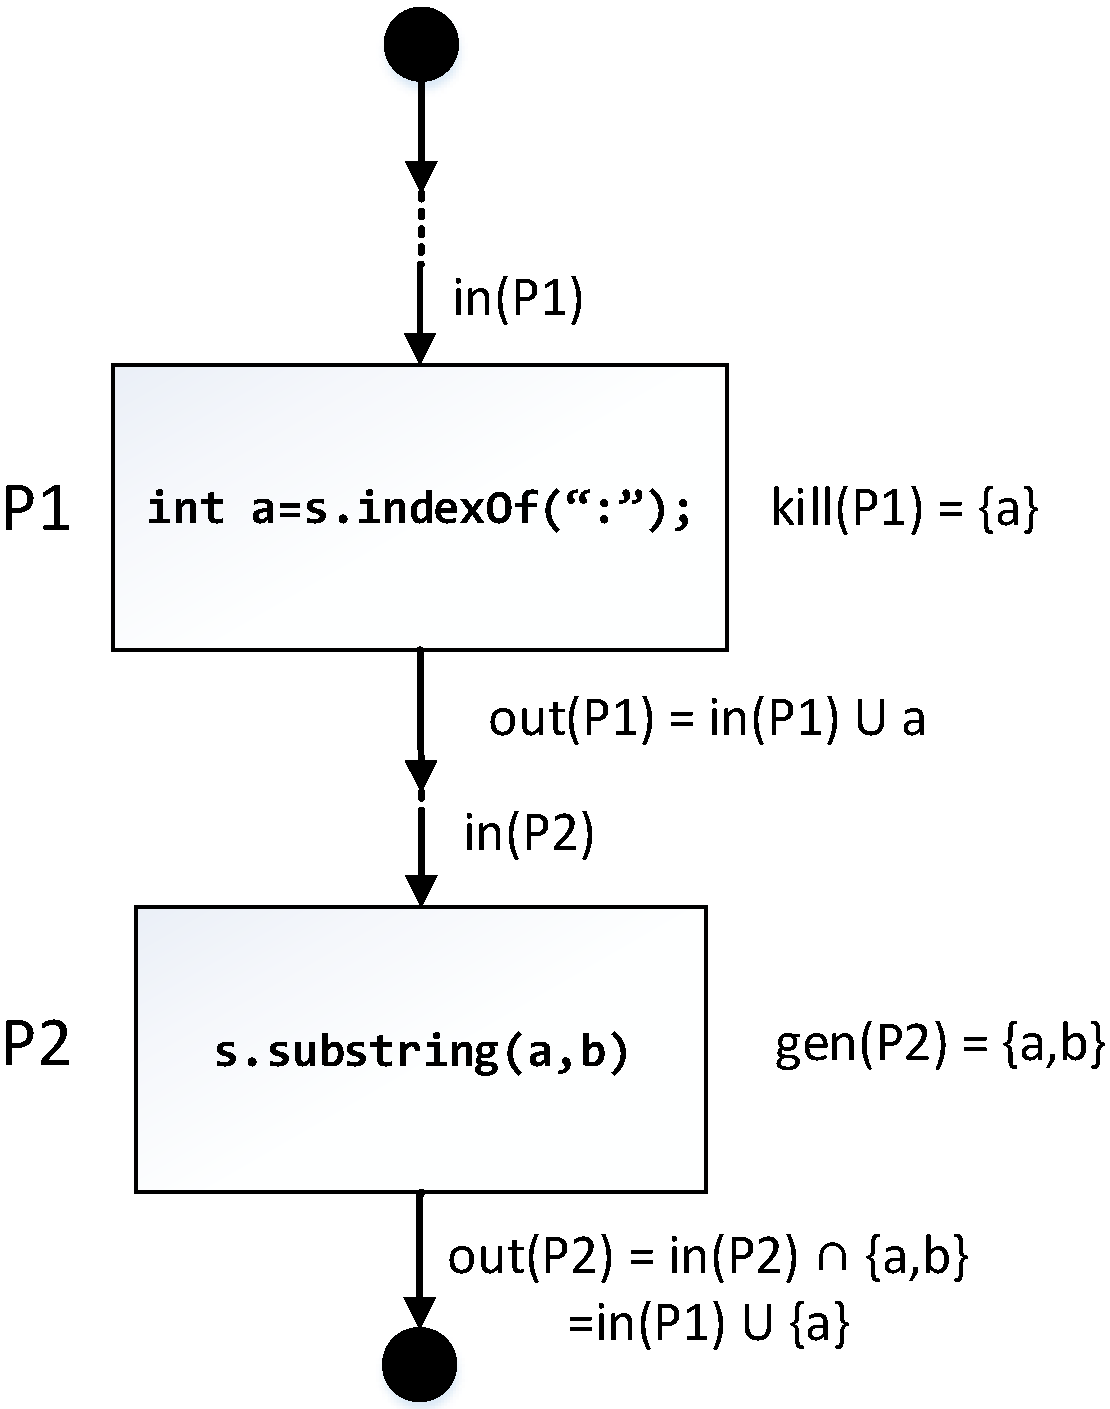
\includegraphics[width=3.2in]{images/dataflow.png}
\caption{Dataflow diagram with in, out set in forward analysis}
\label{fig:dataflow}
\end{figure}

\subsection{Bounded Forward Analysis}
\label{subsec:boundedForward}

Let us define $P_i$ as a program point/ node in the control flow graph. $in(P)$
and $out(P_i)$ respectively denotes in set and out set to and from the node $P$.
We define set $IG$ as the set of methods like \texttt{indexOf()},
\texttt{codePointAt()}, \texttt{CodePointBefore()} etc. which returns an integer
which can be used as input to other String methods. We also define set $IU$
which contains the methods which may use the integers produced by the methods in
$IG$ Then, 
$$out(P_i) = in(P_i) \cup Def(P_i)$$ where statement in P is a invoke statement
and method $m \in IG$ and
$$out(P_i) = in(P_i) \cap Used(P_i)$$ where statement in P is a invoke statement
and method $m \in IU$. Initial entry set = ${\phi}$.


We have defined $Def(P_i)$ set as the set of variables and objects which are
defined or redefined in the program point $P_i$. The set $Used(P_i)$ is also a
set of variables and objects which are used in the program point $P_i$.

\textbf{Example : } Consider the program statement \texttt{Pi : int a = b.fun(c
d)}.
Here the variable \texttt{a} is initialized, so $Def(P_i)$ = \texttt{\{a\}} and
as
\texttt{b, c, d} are used, $Used(P_i) =$ \texttt{\{b, c, d\}}

In the figure~\ref{fig:dataflow}, we gave an example of a sample CFG with in set
and out set.

\subsection{Constraint Satisfaction}
\label{subsec:constraintSatisfaction}

Dataflow analysis plays an important role in preparing the patching. One
patching mechanism we have come up with \texttt{String} objects is tht by
solving constraints which may come up in future will produce patch of better
quality. More over, it is very easy to extend the solution to other objects type
based on their API and characteristics of conditions. One such example is given
in the following code snippet~\ref{snippet:constraintCheck}


\lstset{language=Java, caption=Better patching mechanism with constraint
satisfaction, label = snippet:constraintCheck}
\begin{lstlisting}

void foo(String s, int i, int j)
{
	String str = s.substring(i,j);
	//some operation
	if(str.length() > 12){
	  //do something..
	}
	Integer in = 0;
	try{
	  StreamReader isr = new InputStreamReader(System.in);
	  String sin = new BufferedReader(isr).readLine();
	  in = Integer.parseInt(sin);
	}
	catch(IOException ex){}
	if(str.length() <= in){
	  //do something..
	}
	if(str.startsWith(SomeStringObject)){
	  //do something
	}
}

\end{lstlisting}

In the code snippet~\ref{snippet:constraintCheck}, the statement at line no $4$
is \texttt{s.substring(i,j)}, which can throw a
\texttt{IndexOutOfBoundsException}. This statement requires patching whic
involves generating a string for the object reference \texttt{str}. But in the
progrm, in line numbers \texttt{7, 16} and \texttt{20}, there are threee
conditional statements on \texttt{str} which involves constraint on the length
and the prefix of the string. There may be some set of constraint which can be
evaluated before hand, like the condition in in line numbers \texttt{7} which
involve a constant integer. But there can be cases like the conditional
statement in line numbers \texttt{16} which is also a lenght constraint like the
former, but in involves another variable which is taken frrom console, i.e. the
variable will be evaluated in run time. In such cases we can defer the
constraint evaluation process for that paricular condition. We can evaluate all
the conditions befor it, which can be safely evaluated. When we reach line
number \texttt{16}, then the variable \texttt{tt} would be available and can be
used to reevaluate the string \texttt{str}.

\subsubsection{Constraint Storage}
\label{subsubsec:constraintStorage}

For each of the string object, we store in the way illustrated in the
Figure~\ref{fig:constraint}.

\begin{figure*}[htb]
\centering
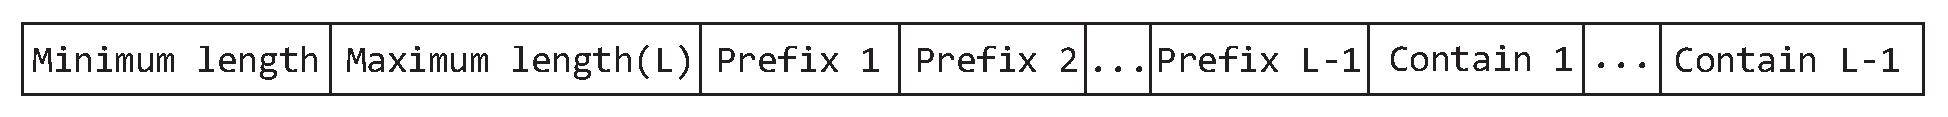
\includegraphics[scale=.5]{images/constraint.eps}
\caption{String constraints storage format}
\label{fig:constraint}
\end{figure*}

Wen to evaluate a new string object we need bounds like the minimuma and maximum
length, the prefixes and the candidate characters and their relative position.
We keep minimum information to safely evaluate the string.

\subsubsection{Constraint Evaluation Strategy}
\label{subsubsec:constraintStorage}

\begin{algorithm}
\DontPrintSemicolon
\KwData{String object $Str$ and constraint set $CS$.}
\KwResult{String object $Str$ such that $\forall i \in CS$, $Str$ satisfies $i$
}
\Begin
{
 $CS_{Str} \longleftarrow$ Get the constrint set for $Str$\;
 $MinLength \longleftarrow CS_{Str}[0]$\;
 $MaxLength \longleftarrow CS_{Str}[1]$\;
 $PrefixSet_{Str} \longleftarrow CS_{Str}[2 \rightarrow MaxLength + 1]$\;
 $ContainSet_{Str} \longleftarrow CS_{Str}[MaxLength +2  \rightarrow 2*MaxLength
 + 1]$\;
 
  \For{$C \in PrefixSet_{Str}$}
  {
   \If{$C$ is Empty}
   {
    continue\;
   }
   $PrefixLength \longleftarrow$ {\bf LENGTH OF} $C$\;
   
   \If{$PrefixLength$ is Maximum $\in PrefixSet_{Str}$}
   {
     Use $C$ to construct $Str$\;
   }
  }
 
  \For{$C \in ContainSet_{Str}$}
  {
   \If{$C$ is Empty {\bf OR} $C \in Str$}
   {
    continue\;
   }
   $Str \leftarrow Str$ {\bf APPEND} $C$\;
  }
  return $Str$\;
}
\caption{String object constraint evaluation}
 \label{algo:constraint}
\end{algorithm}

\subsubsection{Repairing Strategy using Constraint Evaluation}
\label{subsubsec:repairingStrategyConstraint}

The patching is evaluated in two ways, static and dynamic. We evaluated those
conditions which can be evaluated safely during compile time. Such constraints
have constants like \texttt{if(s.length<10)}. We looked for particular
constraints based on our storage specification 
